\let\negmedspace\undefined
\let\negthickspace\undefined
\documentclass[journal]{IEEEtran}
\usepackage[a5paper, margin=10mm, onecolumn]{geometry}
%\usepackage{lmodern} % Ensure lmodern is loaded for pdflatex
\usepackage{tfrupee} % Include tfrupee package

\setlength{\headheight}{1cm} % Set the height of the header box
\setlength{\headsep}{0mm}     % Set the distance between the header box and the top of the text

\usepackage{gvv-book}
\usepackage{gvv}
\usepackage{cite}
\usepackage{amsmath,amssymb,amsfonts,amsthm}
\usepackage{algorithmic}
\usepackage{graphicx}
\usepackage{textcomp}
\usepackage{xcolor}
\usepackage{txfonts}
\usepackage{listings}
\usepackage{enumitem}
\usepackage{mathtools}
\usepackage{gensymb}
\usepackage{comment}
\usepackage[breaklinks=true]{hyperref}
\usepackage{tkz-euclide} 
\usepackage{listings}
\usepackage{tikz}
\usetikzlibrary{patterns}
% \usepackage{gvv}                                        
\def\inputGnumericTable{}                                 
\usepackage[latin1]{inputenc}                                
\usepackage{color}                                            
\usepackage{array}                                            
\usepackage{longtable}                                       
\usepackage{calc}                                             
\usepackage{multirow}                                         
\usepackage{hhline}                                           
\usepackage{ifthen}                                           
\usepackage{lscape}
\begin{document}
\bibliographystyle{IEEEtran}
\vspace{3cm}

\title{GATE\\CE - 2008}
\author{EE24BTECH11061 - Rohith Sai}
\maketitle

\renewcommand{\thefigure}{\theenumi}
\renewcommand{\thetable}{\theenumi}

\section*{Single Correct 1 Mark each}
\begin{enumerate}
\item The capacities of "One-way 1.5 m wide sidewalk (persons per hour)" and "One-way 2-lane urban road (PCU per hour, with no frontage access, no standing vehicles and very little cross traffic)" are respectively
\begin{multicols}{2}
    \begin{enumerate}
        \item 1200 and 2400
        \item 1800 and 2000
        \item 1200 and 1500
        \item 2000 and 1200
    \end{enumerate}
\end{multicols}

\item The shape of the STOP sign according to IRC:67-2001 is
\begin{multicols}{2}
    \begin{enumerate}
        \item circular
        \item triangular
        \item octagonal 
        \item rectangular
    \end{enumerate}
\end{multicols}

\item The type of surveying in which the curvature of the earth is taken into account is called
\begin{multicols}{2}
    \begin{enumerate}
        \item Geodetic surveying
        \item Plane surveying
        \item Preliminary surveying
        \item Topographical surveying
    \end{enumerate}
\end{multicols}

\section*{Single Correct 2 Marks each}
\item The equation $k_x \frac{\partial^2 h}{\partial x^2} + k_z \frac{\partial^2 h}{\partial z^2} = 0$ can be transformed to $\frac{\partial^2 h}{\partial x_{t}^2} + \frac{\partial^2 h}{\partial z^2} = 0$ by substituting
\begin{multicols}{2}
    \begin{enumerate}
        \item $x_t = x \frac{k_z}{k_x}$
        \item $x_t = x \frac{k_x}{k_z}$
        \item $x_t = x \sqrt{\frac{k_x}{k_z}}$
        \item $x_t = x \sqrt{\frac{k_z}{k_x}}$
    \end{enumerate}
\end{multicols}

\item The value of $\int_0^3 \int_0^x \brak{6-x-y}, dx dy$ is
\begin{multicols}{2}
    \begin{enumerate}
        \item 13.5
        \item 27.0
        \item 40.5
        \item 54.0
    \end{enumerate}
\end{multicols}

\item Three values of $x$ and $y$ are to be fitted in a straight line in the form $y = a + bx$ by the method of least squares. Given: $\sum x = 6$, $\sum y = 21$, $\sum x^2 = 14$ and $\sum xy = 46$, the values of $a$ and $b$ are respectively
\begin{multicols}{2}
    \begin{enumerate}
        \item 2 and 3
        \item 1 and 2
        \item 2 and 1
        \item 3 and 2
    \end{enumerate}
\end{multicols}

\item Solution of $\frac{dy}{dx} = -\frac{x}{y}$ at $x=1$ and $y=\sqrt{3}$ is
\begin{multicols}{2}
    \begin{enumerate}
        \item $x-y^2 = -2$
        \item $x + y^2 = 4$
        \item $x^2 - y^2 = -2$
        \item $x^2 + y^2 = 4$
    \end{enumerate}
\end{multicols}

\item If probability density function of a random variable X is 
\begin{align*}
    f\brak{x} = x^2 \text{ for } -1 \leq x \leq 1, \text{ and}
     = 0 \text{ for any other value of $x$}
\end{align*}
then, the percentage probability $P\brak{-\frac{1}{3}} \leq x \leq \frac{1}{3}$ is
\begin{multicols}{2}
    \begin{enumerate}
        \item 0.247
        \item 2.47
        \item 24.7
        \item 247
    \end{enumerate}
\end{multicols}

\item The Eigen values of the matrix $\vec{P} = \myvec{4 & 5 \\ 2 & -5}$ are
\begin{multicols}{2}
    \begin{enumerate}
        \item -7 and 8
        \item -6 and 5
        \item 3 and 4
        \item 1 and 2
    \end{enumerate}
\end{multicols}

\item A person on a trip has a choice between private car and public transport. The probability of using a private car is 0.45 . While using the public transport, further choices available are bus and metro, out of which the probability of commutating by a bus is 0.55. In such a situation, the probability (rounded up to two decimals) of using a car, bus and metro, respectively would be
\begin{multicols}{2}
    \begin{enumerate}
        \item 0.45, 0.30 and 0.25
        \item 0.45, 0.25 and 0.30
        \item 0.45, 0.55 and 0.00
        \item 0.45, 0.35 and 0.20
    \end{enumerate}
\end{multicols}

\item The following simultaneous equations
\begin{align*}
    x + y + z = 3\\
    x + 2y + 3z = 4\\
    x + 4y + kz = 6
\end{align*}
will \textbf{NOT} have a unique solution for $k$ equal to
\begin{multicols}{2}
    \begin{enumerate}
        \item 0
        \item 5
        \item 6
        \item 7
    \end{enumerate}
\end{multicols}

\item The inner (dot) product of two vectors $\vec{P}$ and $\vec{Q}$ is zero. The angle (degrees) between the two vectors is
\begin{multicols}{2}
    \begin{enumerate}
        \item 0
        \item 30
        \item 90
        \item 120
    \end{enumerate}
\end{multicols}

\item Cross-section of a column consisting of two steel strips, each of thickness t and width b is shown in the figure below. The critical loads of the column with perfect bond and without bond between the strips are $P$ and $P_0$ respectively. The ratio $\frac{P}{P_0}$
\begin{tikzpicture}

% First rectangle (top, shaded with north-east lines)
\fill[pattern=north east lines] (0,1) rectangle (3.5,2);
\draw (0,1) rectangle (3.5,2);

% Second rectangle (bottom, shaded with north-west lines)
\fill[pattern=north west lines] (0,0) rectangle (3.5,1);
\draw (0,0) rectangle (3.5,1);

% Label for 'b' below the rectangles, keeping the length the same
\draw[<->] (0,-0.5) -- (3.5,-0.5) node[midway,below] {$b$};

% First 't' on the right side of the first (top) rectangle
\draw[<->] (3.7,1) -- (3.7,2) node[midway,right] {$t$};

% Second 't' on the right side of the second (bottom) rectangle
\draw[<->] (3.7,0) -- (3.7,1) node[midway,right] {$t$};

\end{tikzpicture}
\begin{multicols}{2}
    \begin{enumerate}
        \item 2
        \item 4
        \item 6
        \item 8
    \end{enumerate}
\end{multicols}

\item A rigid bar GH of length L is supported by a hinge and a spring of stiffness K as shown in the figure below. The buckling load $P_{Cr}$, for the bar will be
\begin{tikzpicture}

% Coordinates
\coordinate (H) at (0,0);  % Point H
\coordinate (G) at (0,-5); % Point G directly below H
\coordinate (K) at (2,0);  % Point K to the right, above the center of the spring

% Vertical rod (L)
\draw[thick] (H) -- (G);

% Ground at G (triangle)
\draw[thick] (G) -- (-0.5,-5.5) -- (0.5,-5.5) -- cycle;
\fill[gray!30] (-0.5,-5.5) -- (0.5,-5.5) -- (G) -- cycle; % Shading below triangle

% Circle joints at H and G
\draw[fill=white, thick] (H) circle (3pt); % Joint at H
\draw[fill=white, thick] (G) circle (3pt); % Joint at G

% Label G to the left of the circle at G
\node at (-0.3,-5) {$G$};

% Spring from H to K (right side, increased length)
\draw[thick] (H) -- (K); % Connecting line from H to K
\draw[thick,decorate,decoration={coil,aspect=0.8,amplitude=5pt,segment length=5pt}] (K) -- ++(1.5,0);

% Force arrow P at H
\draw[thick,->] (0,0.5) -- (0,0); % Arrow pointing down at H
\node at (0.2,0.3) {$P$}; % Label P at the tail of the arrow

% Fixed wall at K (right side)
\draw[thick] (3.5,-0.5) -- (3.5,0.5); % Wall vertical
\draw[thick] (3.5,-0.5) -- (4,-0.5) -- (4,0.5) -- (3.5,0.5); % Horizontal lines
\fill[gray!30] (3.5,-0.5) rectangle (4,0.5); % Shading to the right of the rectangle

% Labels
\node at (0.2,-2.5) {$L$};  % Label for length L
\node at (2.5,0.5) {$K$};   % Label for K, directly above the center of the spring
\node at (-0.3,0.2) {$H$};  % Label for H

\end{tikzpicture}

\begin{multicols}{2}
    \begin{enumerate}
        \item 0.5 KL
        \item 0.8 KL
        \item 1.0 KL
        \item 1.2 KL
    \end{enumerate}
\end{multicols}

\item The degree of static indeterminacy of the rigid frame having two internal hinges as shown in the figure below is:

\begin{tikzpicture}

% Coordinates for the structure
\coordinate (H) at (0,0);   % Point H
\coordinate (I) at (2,0);   % Point I
\coordinate (J) at (4,0);   % Point J
\coordinate (G) at (0,-2);  % Support G
\coordinate (F) at (2,-2);  % Support F
\coordinate (E) at (4,-2);  % Support E

% Horizontal beams
\draw[thick] (H) -- (I);  % H to I
\draw[thick] (I) -- (J);  % I to J

% Vertical beams
\draw[thick] (H) -- (G);  % H to G
\draw[thick] (I) -- (F);  % I to F
\draw[thick] (J) -- (E);  % J to E
\draw[thick] (G) -- (F);  % G to F
\draw[thick] (F) -- (E);  % F to E

% Supports at G, F, and E
% Fixed support at G (triangle outline without shading)
\draw[thick] (G) -- (-0.5,-2.5) -- (0.5,-2.5) -- cycle; % Outline of triangle G

% Adding rectangle hash shading below triangle G
\fill[pattern=north east lines] (-0.5,-2.8) rectangle (0.5,-2.5); % Hash shading for the rectangle below triangle G

% Roller support at F (triangle with a line below)
\draw[thick] (F) -- (1.5,-2.5) -- (2.5,-2.5) -- cycle;
\draw[thick] (1.5,-2.5) -- (2.5,-2.5); % Ground line under triangle

% Roller support at E (triangle with a line below)
\draw[thick] (E) -- (3.5,-2.5) -- (4.5,-2.5) -- cycle;
\draw[thick] (3.5,-2.5) -- (4.5,-2.5); % Ground line under triangle

% Adding wheels at the bottom vertices of triangles F and E
\draw[fill=white, thick] (1.5,-2.5) circle (3pt); % Wheel 1 at F
\draw[fill=white, thick] (2.5,-2.5) circle (3pt); % Wheel 2 at F
\draw[fill=white, thick] (3.5,-2.5) circle (3pt); % Wheel 1 at E
\draw[fill=white, thick] (4.5,-2.5) circle (3pt); % Wheel 2 at E

% Circle joints at H, I, and J
\draw[fill=white, thick] (1.5, 0) circle (3pt);  % Joint at H and I
\draw[fill=white, thick] (2.5, 0) circle (3pt);  % Joint at I and J

% Line to the circles
\draw[thick] (1.5, -2.6) -- (2.5, -2.6);
\draw[thick] (3.5, -2.6) -- (4.5, -2.6);

% Labels for points H, I, J, G, F, and E
\node at (-0.3,0.2) {H};   % Label H
\node at (2,0.2) {I};    % Label I
\node at (4,0.2) {J};    % Label J
\node at (-0.3,-1.75) {G};  % Label G
\node at (1.7,-1.75) {F};   % Label F
\node at (3.7,-1.75) {E};   % Label E

\end{tikzpicture}
\begin{multicols}{2}
    \begin{enumerate}
        \item 8
        \item 7
        \item 6
        \item 5
    \end{enumerate}
\end{multicols}

\item The members $EJ$ and $IJ$ of a steel truss shown in the figure below are subjected to a temperature rise of $30\degree $C. The coefficient of thermal expansion of steel is 0.000012 per $\degree$C per unit length. The displacement (mm) of joint $\vec{E}$ relative to joint $\vec{H}$ along the direction $HE$ of the truss, is\\
\begin{tikzpicture}

% Points
\coordinate (G) at (0,0);     % Point G
\coordinate (H) at (3,0);     % Point H
\coordinate (I) at (6,0);     % Point I
\coordinate (E) at (0,3);     % Point E
\coordinate (J) at (3,3);     % Point J

% Draw the structure
\draw[thick] (G) -- (E);     % Join G and E
\draw[thick] (G) -- (H);     % Join G and H
\draw[thick] (H) -- (I);     % Join H and I
\draw[thick] (E) -- (J);     % Join E and J
\draw[thick] (H) -- (J);     % Vertical member
\draw[thick] (J) -- (I);     % Join J and I
\draw[thick] (G) -- (J);     % Join G and J

% Supports
\draw[thick] (G) -- ++(-0.3,-0.3) -- ++(0.6,0) -- ++(-0.3,0.3); % Fixed support at G
\draw[thick] (I) -- ++(-0.3,-0.3) -- ++(0.6,0) -- ++(-0.3,0.3);
\draw[fill=white, thick] (5.7,-0.3) circle (3pt);
\draw[fill=white, thick] (6.3,-0.3) circle (3pt);
\draw[thick] (5.7,-0.4) -- (6.3,-0.4);

% Labels
\node[above left] at (G) {G};  % Label G
\node[below right] at (H) {H}; % Label H
\node[above right] at (I) {I}; % Label I
\node[above] at (J) {J};       % Label J
\node[above] at (E) {E};       % Label E

% shade
\fill[pattern=north east lines] (-0.3,-0.3) rectangle (0.3,-0.5);

% Dimension lines (outside the figure)
\draw[<->, thick] (0, -0.75) -- (3, -0.75) node[midway, below] {3000 mm}; % G-H
\draw[<->, thick] (3, -0.75) -- (6, -0.75) node[midway, below] {3000 mm}; % H-I
\draw[<->, thick] (-0.75, 0) -- (-0.75, 3) node[midway, left] {3000 mm};  % G-E

\end{tikzpicture}

\begin{multicols}{2}
    \begin{enumerate}
        \item 0.255
        \item 0.589
        \item 0.764
        \item 1.026
    \end{enumerate}
\end{multicols}

\item The maximum shear stress in a solid shaft of circular cross-section having diameter d subjected to a torque T is $\tau$. If the torque is increased by four times and the diameter of the shaft is increased by two times, the maximum shear stress in the shaft will be
\begin{multicols}{2}
    \begin{enumerate}
        \item $2\tau$
        \item $tau$
        \item $\frac{\tau}{2}$
        \item $\frac{\tau}{4}$
    \end{enumerate}
\end{multicols}
\end{enumerate}
\end{document}